% this file is called up by thesis.tex
% content in this file will be fed into the main document

%: ----------------------- name of chapter  -------------------------
\chapter{Experimental Platforms}
% top level followed by section, subsection
\label{appx:exp_platform}
%: ----------------------- paths to graphics ------------------------

% change according to folder and file names
\ifpdf
    \graphicspath{{A_experimental_platform/figures/PNG/}{A_experimental_platform/figures/PDF/}{A_experimental_platform/figures/}}
\else
    \graphicspath{{A_experimental_platform/figures/EPS/}{A_experimental_platform/figures/}}
\fi



The experimental validation of the framework proposed in this thesis has
involved two \acp{AUV}. While most of those tests were conducted with the
Sparus~II \ac{AUV}, the experiments that proved one of the framework
capabilities were done with the AsterX \ac{AUV}. The following sections explain
the main software and hardware aspects of both vehicles.

\section{Sparus II AUV}

The Sparus~II is a torpedo-shaped \ac{AUV} with hovering capabilities, which has
been designed and developed at the
\ac{CIRS}\footnote{\href{http://cirs.udg.edu/}{CIRS} is part of the \ac{ViCOROB}
in Girona (Spain)}. The vehicle is rated for depths up to $200 m$, and is
equipped with three thrusters; two of them are located in the back, and are used
for motion on the horizontal plane; the third one is located in the middle, and
is dedicated to vertical motion. This implies that the \ac{AUV} can be actuated
in surge, heave and yaw \ac{DOF}. Furthermore, the Sparus~II is equipped with a
navigation sensor suite that includes a pressure sensor, a \acf{DVL}, an
\acf{IMU} and a GPS to receive position fixes while at surface. 

The Sparus~II \ac{AUV} also has communication devices such as an acoustic modem
for underwater communication with other vehicles or surface stations (\eg by
using an \ac{USBL} system), and a Wi-Fi antenna that can be used when the
\ac{AUV} is at surface. Moreover, the vehicle includes a configurable payload
area in the front, which contains a set of exteroceptive sensors to perceive and
detect the surroundings. This latter group of sensors can be modified according
to the mission's requirements, and may include optical cameras, single-beam
echosounders, mechanical-scanning (profiler and imaging) sonars, multibeam
sonars, etc. Figure~\ref{fig:Sparus2FullViews} depicts different views of the
Sparus~II \ac{AUV}, including one where a possible payload configuration can be
observed.


\begin{figure}[htbp]
    \myfloatalign
    \subfloat[Sparus~II in a water tank at \ac{CIRS}]
    {\label{fig:Sparus2FullReal}%
     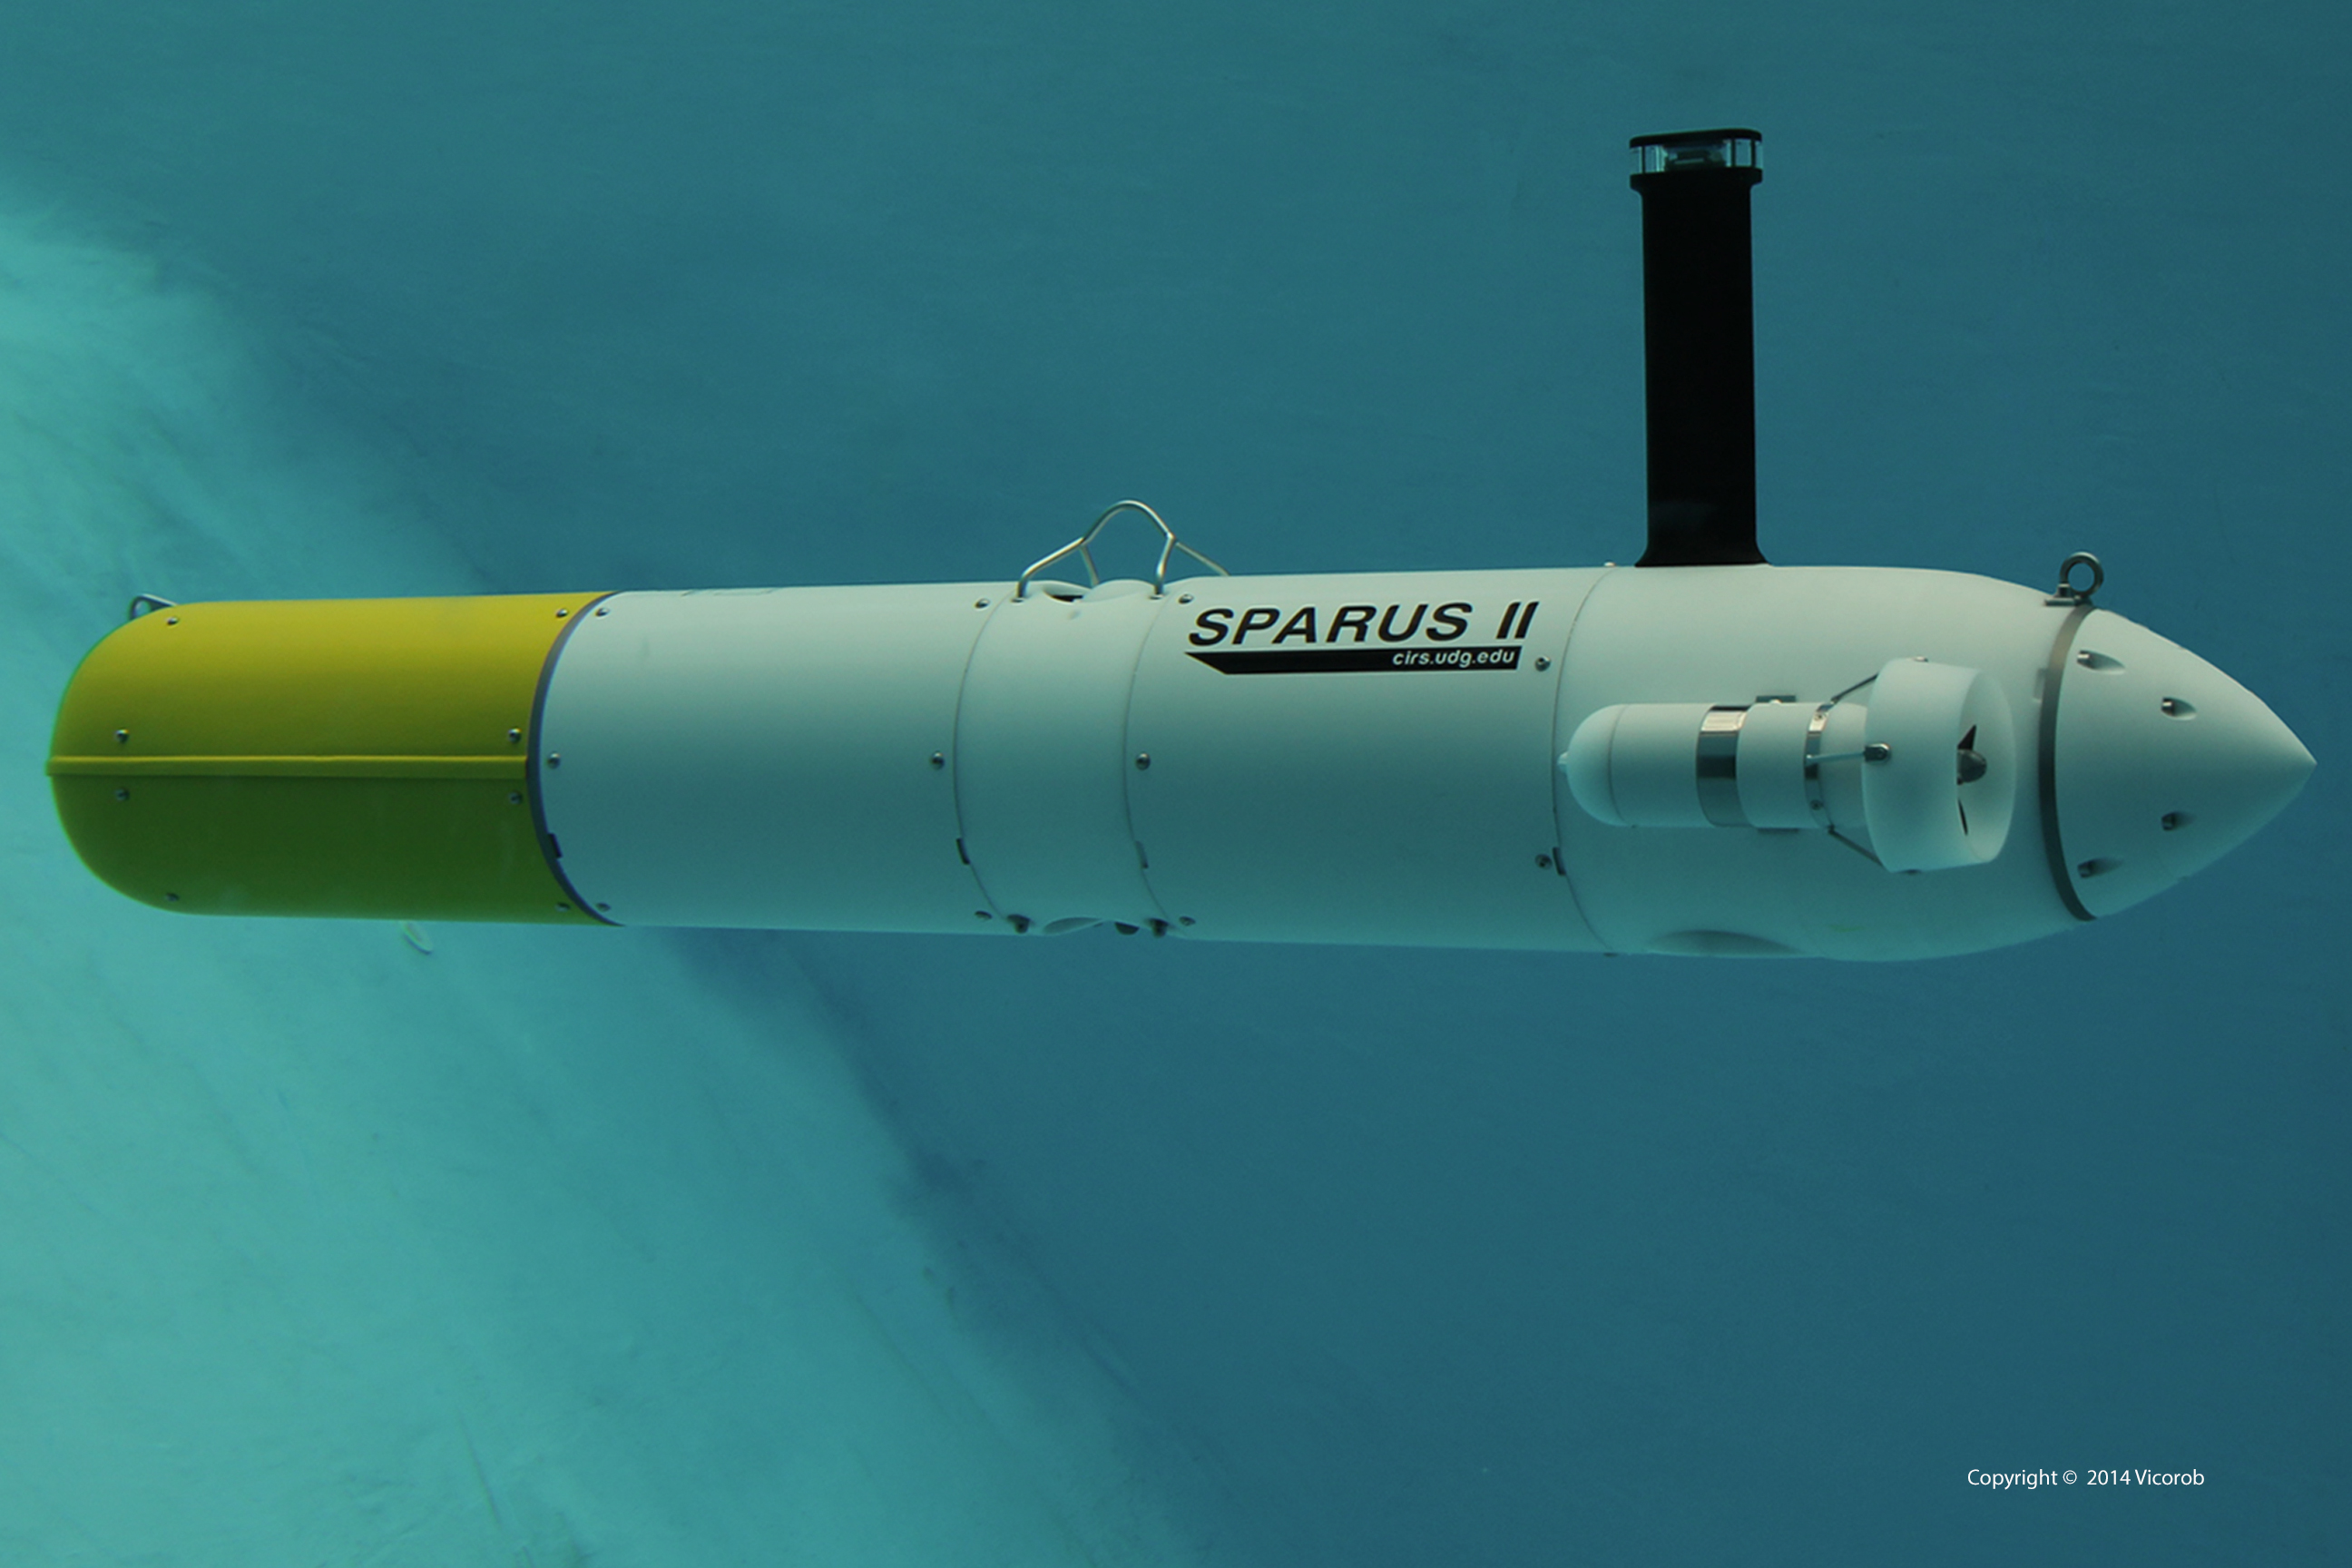
\includegraphics[width=.65\linewidth]{Sparus2FullReal}}\\
    \subfloat[Top view]
    {\label{fig:Sparus2FullTop}
    \includegraphics[width=.65\linewidth]{Sparus2FullTop}} \\%\quad
    \subfloat[Bottom view]
    {\label{fig:Sparus2FullBottom}%
     \includegraphics[width=.65\linewidth]{Sparus2FullBottom}}\\
    \subfloat[Lateral view]
    {\label{fig:Sparus2FullLateral}
    \includegraphics[width=.65\linewidth]{Sparus2FullLateral}}\\ %\quad
    \subfloat[3D view]
    {\label{fig:Sparus2Full3D}%
     \includegraphics[width=.65\linewidth]{Sparus2Full3D}}
    \caption[Sparus~II AUV: top, bottom, lateral and 3D views, and its hardware
    elements.] 
    {Sparus~II AUV: top, bottom, lateral and 3D views. Different hardware parts
    can be observed, including the thrusters (1,2), the acoustic modem (3), the
    Wi-Fi and GPS (4), as well as interoceptive and exteroceptive sensors such
    as the DVL (5), side-scan sonar (6), mechanically-scanning imaging sonar
    (7), single-beam echosounders (8), multibeam sonar (9), and an optical
    camera (10).}
    \label{fig:Sparus2FullViews}
\end{figure}

In what software concerns, the Sparus~II \ac{AUV} is controlled through the
\acf{COLA2}~\cite{Palomeras2012}, which is a control architecture that is
completely integrated with the \acf{ROS}. Besides operating aboard real robots,
\ac{COLA2} can interact with the \acf{UWSim}~\cite{Prats2012}, which can import
\ac{3D} environment models and simulate the vehicle's sensors and dynamics with
high fidelity. Furthermore, the use of \ac{ROS} allows to easily integrate third
party tools, such as the \acf{OMPL} that offers a convenient framework that can
be adapted to specific path/motion planning problems~\cite{Sucan2012}.

% \begin{figure}[htbp]
% 	\centering
% 	\includegraphics[width=.85\linewidth]{MicronAperture} 
% 	\caption{\hl{Micron} Aperture.}
% 	\label{fig:MicronAperture}
% \end{figure}

\section{AsterX AUV}

The AsterX is a torpedo-shaped \ac{AUV} from the \acf{Ifremer}. This vehicle is
based on the Explorer~3000 \ac{AUV}, which is built by \ac{ISE}, from Canada.
The vehicle is rated for depths up to $3000 m$, and is equipped with one back
propulsion motor, three aft steering planes, and two fore planes. Similarly as
the Sparus~II, AsterX is equipped with a navigation sensor suite that includes a
pressure sensor, a \ac{DVL}, an \ac{IMU} and a GPS to receive position fixes
while at surface. It also has an acoustic modem, and a Wi-Fi antenna. This
\ac{AUV} also includes a modular payload area in the front, which may carry
different sensors, \eg a multibeam sonar. Figure~\ref{fig:AsterXFullViews}
depicts the AsterX \ac{AUV} at sea surface, and a schematic with its main inner
hardware devices distribution.

\begin{figure}[htbp]
    \myfloatalign
    \subfloat[AsterX \ac{AUV} at sea surface during in-water trials]
    {\label{fig:AsterXFullReal}%
     \includegraphics[width=.65\linewidth]{AsterXFullReal}}\\
%     \subfloat[Top view]
%     {\label{fig:AsterXFullTop}
%     \includegraphics[width=.65\linewidth]{AsterXFullTop}} \\%\quad
    \subfloat[Lateral view]
    {\label{fig:AsterXFullLateral}
    \includegraphics[width=.65\linewidth]{AsterXFullLateral}}\\ %\quad
    \caption[AsterX AUV at sea surface and its lateral view with a description of the
    different hardware elements.]
    {AsterX AUV at sea surface and its lateral view with a description of the
    different hardware elements.}
    \label{fig:AsterXFullViews}
\end{figure}

On the other hand, the AsterX's software architecture is composed of
three main functional blocks (see Fig.~\ref{fig:HighLevelControArch}).  Firstly,
the \ac{AUV} low-level controller, also referred as \textit{frontseat}, guides
the vehicle using the \ac{ACE} middleware. This controller is executed over QNX
operating system, thus guaranteeing real-time computation constraints.
Furthermore, this functional block also handles the vehicle's navigation and
safety routines. Secondly, the \textit{backseat} controller extends the
vehicle's capabilities and applications by easing the implementation of
high-level routines, such as algorithms for path/motion planning, path-tracking,
and docking. These routines can directly send low-level control setpoints. This
functional block has its own dedicated computer that works under the \ac{ROS}
(over Linux). Finally, the \textit{payload} controller acts as a bidirectional
interface between the interoceptive and exteroceptive sensors, and, on the other
hand, both the \textit{frontseat} and \textit{backseat} controllers.

\begin{figure}[htbp] %  figure placement: here, top, bottom, or page
\centering
	\includegraphics[width=.7\linewidth]{AsterX-Software-Architecture}
\caption[AsterX AUV software architecture.]
{AsterX \ac{AUV} software architecture}
\label{fig:HighLevelControArch}
\end{figure}
